\subsection{点云后处理模块}
\par 该模块对输入的点云数据,包含每个点的全局三维坐标、RGB值和类别标签进行处理,组件图如图\ref{fig:component6}所示,时序图如图\ref{fig:sequence7}所示。

\begin{figure}[htb]
	\centering
	\begin{minipage}[t]{0.42\textwidth}
		\centering
		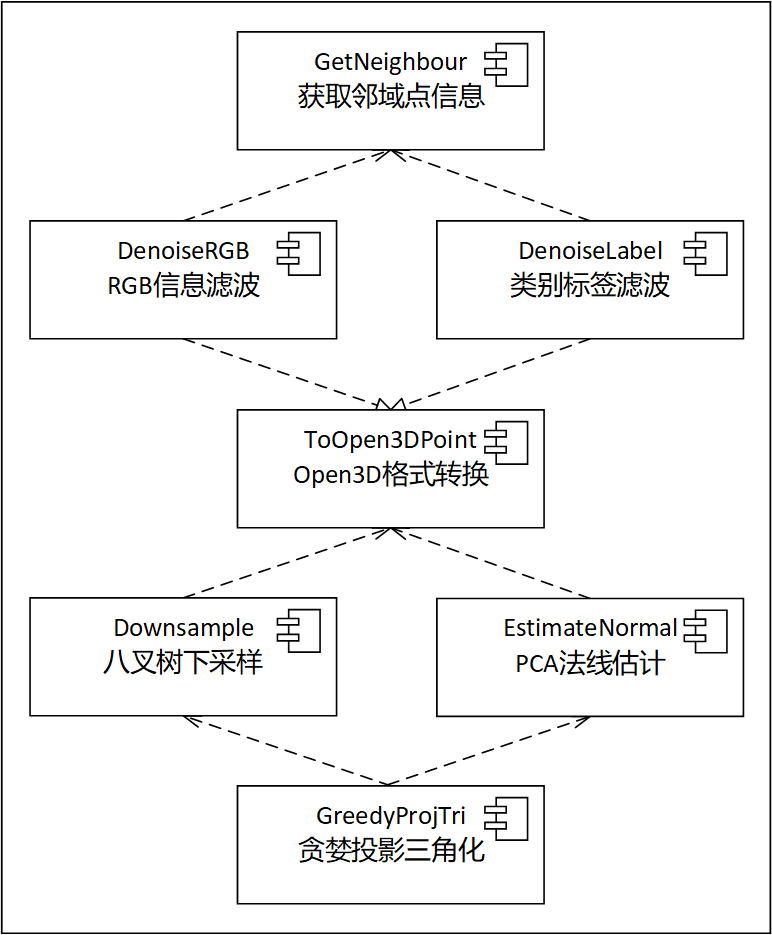
\includegraphics[height=7.5cm,keepaspectratio]{figures/uml/component6.png}
		\caption{点云后处理模块组件图}
		\label{fig:component6}
	\end{minipage}
	\begin{minipage}[t]{0.53\textwidth}
		\centering
		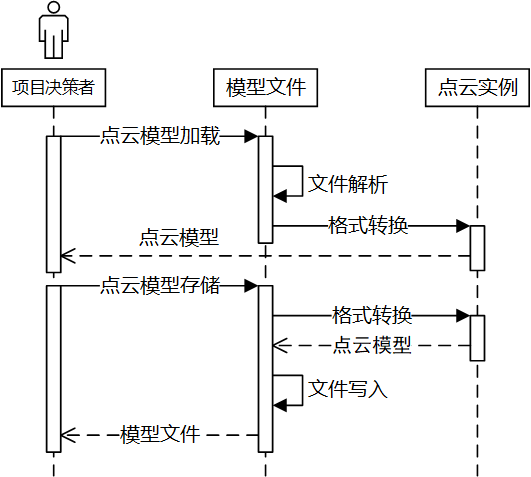
\includegraphics[height=7.5cm,keepaspectratio]{figures/uml/sequence7.png}
		\caption{模型导入导出模块时序图}
		\label{fig:sequence7}
	\end{minipage}
\end{figure}

\par 点云模型重建完成后,首先进行点云的降噪操作。在室内重建中,由于噪声点和离群点的存在,
会对模型质量产生影响。因此,使用基于局部密度的滤波方法进行降噪可以在去除噪声的同时保留边缘
信息。\texttt{Space}类定义了函数\texttt{GetNeighbour}、\texttt{DenoiseRGB}和\texttt{DenoiseLabel},用于获取点的邻域信息并且
对点的RGB值和类别标签进行滤波处理,邻域点集类别标签的多数可以由算法\ref{algo:GetMajorityLabel}得到,每个点的序号可以由公式\ref{get_neighbour}计算出:
\begin{equation}
	\begin{aligned}
		& \texttt{Left}   &  & = (\texttt{blockIdx} \times \texttt{blockDim} + \texttt{threadIdx}) \times \texttt{n} + \texttt{i} - 1       \\
		& \texttt{Right}  &  & = (\texttt{blockIdx} \times \texttt{blockDim} + \texttt{threadIdx}) \times \texttt{n} + \texttt{i} + 1       \\
		& \texttt{Up}     &  & = (\texttt{blockIdx} \times \texttt{blockDim} + \texttt{threadIdx} + 1) \times \texttt{n} + \texttt{i}       \\
		& \texttt{Down}   &  & = (\texttt{blockIdx} \times \texttt{blockDim} + \texttt{threadIdx} - 1) \times \texttt{n} + \texttt{i}       \\
		& \texttt{Front}  &  & = ((\texttt{blockIdx} + 1) \times \texttt{blockDim} + \texttt{threadIdx}) \times \texttt{n} + \texttt{i} - 1 \\
		& \texttt{Behind} &  & = ((\texttt{blockIdx} - 1) \times \texttt{blockDim} + \texttt{threadIdx}) \times \texttt{n} + \texttt{i} - 1 \\
	\end{aligned}
	\label{get_neighbour}
\end{equation}
其中,$\texttt{n}$ 为点云数组 $\texttt{point\_list}$ 的长度,$\texttt{i}$ 为当前点在点云数组中的序号。

\begin{algorithm}[htb]
	\SetAlgoLined
	\KwData{领域点集 neighbor\_point[], 类别标签集合 list[]}
	\KwResult{多数标签 majority\_label}
	初始化整数数组 $count[27]$ 用于计算领域点集标签的数量\;
	初始化 $num = 0$\;
	\For{$i$ in 领域点集中所有的点}{
		\If{not $neighbor\_point[i]$}{
			继续下一次循环\;
		}
		$count[int(list[i])]++$\;
		\If{$count[int(list[i])] > num$}{
			$num = count[int(list[i])]$\;
			$majority\_label = list[i]$\;
		}
	}
	\caption{GetMajorityLabel}
	\label{algo:GetMajorityLabel}
\end{algorithm}

\par 降噪完成后,可选择进行点云的下采样、法线估计和曲面重建操作。为了更好地实现这些功能,
系统通过\texttt{ToOpen3DPointCloud}把点云数据转换成Open3D库可以处理的格式。函数遍历\texttt{point\_list}数组中所
有的点。对于每个点,它将点的世界坐标 $P_w$ 添加到\texttt{points}数组,将点的RGB值添加到\texttt{colors}数组。

\par \texttt{Downsample}实现了基于八叉树的下采样方法。首先,使用Open3D的\texttt{VoxelDownSample}
方法对点云进行下采样,得到\texttt{voxel\_down\_pcd}点云。接着,清空原始点云\texttt{pcd}的\texttt{points}和\texttt{colors}
数组。然后,遍历下采样后的点云,将每个点的坐标和颜色添加到原始点云\texttt{pcd}中。这一步骤可以
有效地降低点云数据的规模,减少存储和计算成本,同时保留了点云的主要结构信息。

% \begin{figure}[htb]
% 	\centering
% 	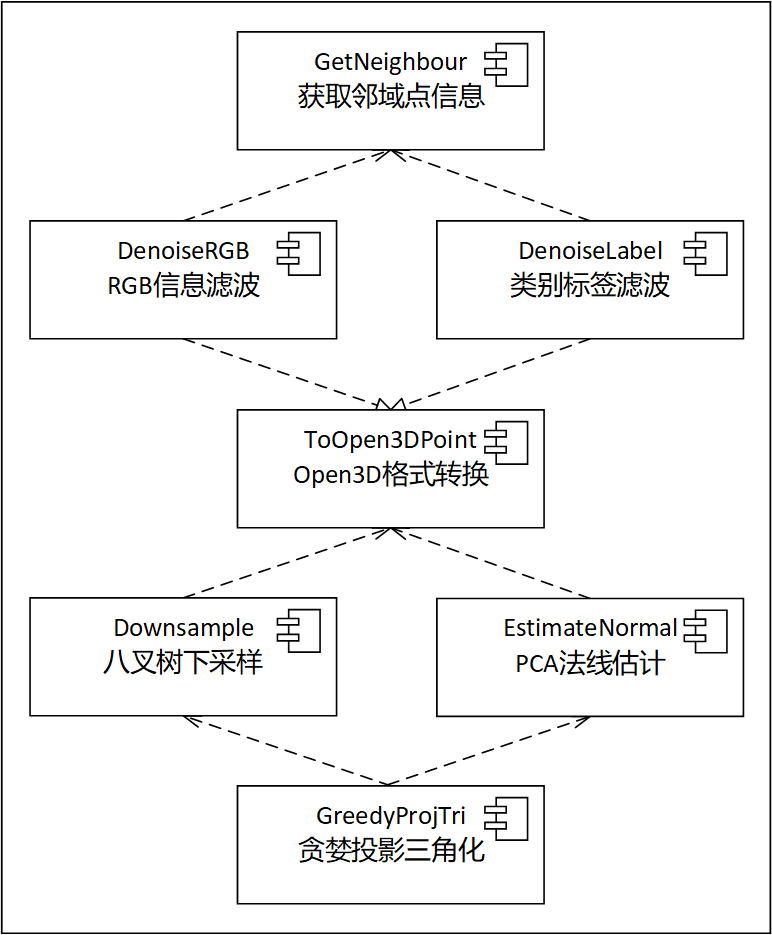
\includegraphics[width=0.7\textwidth]{figures/uml/component6.png}
% 	\caption{点云后处理模块组件图}
% 	\label{fig:component6}
% \end{figure}

% \begin{figure}[htbp]
% 	\centering
% 	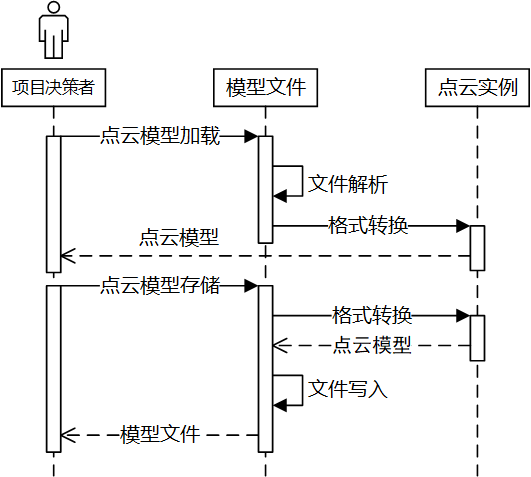
\includegraphics[width=0.618\textwidth]{figures/uml/sequence7.png}
% 	\caption{模型导入导出模块时序图}
% 	\label{fig:sequence7}
% \end{figure}



\par 下采样操作完成后,可以根据需要选择进行表面法线的估计。\texttt{EstimateNormal}实现了基于主成分
分析的法线估计方法。首先,初始化一个协方差矩阵和质心向量。然后,对邻居点进行遍历,
累加每个点的坐标,得到总坐标值后计算平均坐标,也就是质心。接着,再次遍历邻居点,计算每个点
的坐标减去质心的差,然后将其外积添加到协方差矩阵。最后,使用主成分分析算法求解协方差矩阵的特征向
量和特征值,返回特征值最小对应的特征向量,即为点云的法线。

\par 最后,可以选择进行曲面的重建操作。\texttt{GreedyProjTri}调用Open3D库的
\texttt{create\_from\_point\_cloud\_poisson}方法,通过贪婪投影三角化的算法,在给定的半径和最大最近邻距离参数下,对点云进行
三角化处理,生成并返回一个三角形网格。
